% ══════════════════════════════════════════════════════════════════
% smoltcp Quality Assessment – Presentation Slides
% Compile with: pdflatex slides.tex
% ══════════════════════════════════════════════════════════════════
\documentclass[aspectratio=169,11pt]{beamer}

% ── Theme & Colors ──
\usetheme{default}
\usecolortheme{default}
\usepackage[T1]{fontenc}
\usepackage{lmodern}
\usepackage{graphicx}
\usepackage{booktabs}
\usepackage{tabularx}
\usepackage{tikz}
\usepackage{xcolor}
\usepackage{amsmath}
\usetikzlibrary{calc,backgrounds,positioning,shapes.geometric}

% ── Green palette ──
\definecolor{deepgreen}{HTML}{064E3B}
\definecolor{maingreen}{HTML}{059669}
\definecolor{lightgreen}{HTML}{6EE7B7}
\definecolor{palegreen}{HTML}{D1FAE5}
\definecolor{mintbg}{HTML}{ECFDF5}
\definecolor{darktext}{HTML}{1B1B1B}
\definecolor{subtletext}{HTML}{4B5563}
\definecolor{accentlime}{HTML}{A7F3D0}
\definecolor{warnorange}{HTML}{F59E0B}
\definecolor{alertred}{HTML}{EF4444}

% ── Beamer customisation ──
\setbeamercolor{background canvas}{bg=white}
\setbeamercolor{normal text}{fg=darktext}
\setbeamercolor{frametitle}{fg=deepgreen}
\setbeamercolor{title}{fg=white}
\setbeamercolor{subtitle}{fg=accentlime}
\setbeamercolor{item}{fg=maingreen}
\setbeamercolor{itemize item}{fg=maingreen}
\setbeamercolor{itemize subitem}{fg=maingreen!70}
\setbeamercolor{block title}{bg=maingreen,fg=white}
\setbeamercolor{block body}{bg=palegreen,fg=darktext}
\setbeamercolor{block title alerted}{bg=alertred,fg=white}
\setbeamercolor{block body alerted}{bg=alertred!10,fg=darktext}

\setbeamerfont{frametitle}{size=\Large,series=\bfseries}
\setbeamerfont{title}{size=\huge,series=\bfseries}
\setbeamerfont{subtitle}{size=\large}

% ── Remove ALL navigation / footers ──
\beamertemplatenavigationsymbolsempty
\setbeamertemplate{footline}{}
\setbeamertemplate{headline}{}

% ── Custom frametitle with green accent bar (left margin, not overlapping text) ──
\setbeamertemplate{frametitle}{%
  \vskip6pt%
  \hbox{%
    
\begin{tikzpicture}[baseline=(bar.center)]
      \node[inner sep=0pt,outer sep=0pt] (bar) {%
        \textcolor{maingreen}{\rule{3pt}{1.1em}}%
      };
    \end{tikzpicture}%
    \hspace{6pt}%
    \usebeamerfont{frametitle}\usebeamercolor[fg]{frametitle}\insertframetitle%
  }%
  \vskip3pt%
  
\begin{tikzpicture}
    \draw[lightgreen, line width=1pt] (0,0) -- (\textwidth,0);
  \end{tikzpicture}%
  \vskip2pt%
}

% ── Itemize bullets ──
\setbeamertemplate{itemize item}{\textcolor{maingreen}{\raisebox{0.15ex}{\scriptsize$\blacksquare$}}}
\setbeamertemplate{itemize subitem}{\textcolor{maingreen!60}{\raisebox{0.15ex}{\tiny$\blacksquare$}}}

% ── Figures path ──
\graphicspath{{figures/}}

% ══════════════════════════════════════════════════════════════════
\begin{document}

% ─────────────────────── SLIDE 1 : TITLE ───────────────────────
{
\setbeamertemplate{background}{%
  \begin{tikzpicture}[remember picture,overlay]
    \fill[deepgreen] (current page.south west) rectangle (current page.north east);
    \fill[maingreen,opacity=0.25] (current page.north east) ++(-3cm,-2cm) circle (5cm);
    \fill[lightgreen,opacity=0.15] (current page.south west) ++(4cm,3cm) circle (6cm);
    \fill[accentlime,opacity=0.10] (current page.north west) ++(2cm,-5cm) circle (3.5cm);
    \fill[lightgreen,opacity=0.4] (current page.south west) rectangle ([yshift=0.35cm]current page.south east);
  \end{tikzpicture}%
}
\begin{frame}[plain]
  \vspace{1.8cm}
  \centering
  {\usebeamerfont{title}\usebeamercolor[fg]{title} Quality Assessment \& Improvement\\[0.3cm]
  of the \textbf{smoltcp} TCP/IP Stack\par}
  \vspace{0.6cm}
  {\usebeamerfont{subtitle}\usebeamercolor[fg]{subtitle} Security Testing \& Software Quality Assurance\par}
  \vspace{0.4cm}
  {\color{accentlime}\small smoltcp v0.12.0 --- Open-Source Embedded Network Stack\par}
  \vspace{1.2cm}
  {\color{white!80}\small Final Project Presentation~|~April 2026\par}
\end{frame}
}

% ─────────────────────── SLIDE 2 : AGENDA ───────────────────────
\begin{frame}{Agenda}
\begin{columns}[T]
\begin{column}{0.48\textwidth}
  \begin{enumerate}
    \item[\textcolor{maingreen}{\textbf{1}}] Introduction \& Scope
    \item[\textcolor{maingreen}{\textbf{2}}] Mutation Adequacy Testing
    \item[\textcolor{maingreen}{\textbf{3}}] Input Space Partitioning
    \item[\textcolor{maingreen}{\textbf{4}}] Security Fuzzing
    \item[\textcolor{maingreen}{\textbf{5}}] Conformance Testing
  \end{enumerate}
\end{column}
\begin{column}{0.48\textwidth}
  \begin{enumerate}
    \item[\textcolor{maingreen}{\textbf{6}}] Performance Testing
    \item[\textcolor{maingreen}{\textbf{7}}] White-Box Coverage
    \item[\textcolor{maingreen}{\textbf{8}}] Software Safety
    \item[\textcolor{maingreen}{\textbf{9}}] Quality Dashboard
    \item[\textcolor{maingreen}{\textbf{10}}] Conclusions
  \end{enumerate}
\end{column}
\end{columns}
\end{frame}

% ─────────────────────── SLIDE 3 : INTRODUCTION ───────────────────────
\begin{frame}{Introduction}
\begin{block}{What is smoltcp?}
A standalone, event-driven TCP/IP stack written in \textbf{Rust}, targeting embedded, bare-metal, and resource-constrained systems.
\end{block}
\vspace{0.3cm}
\begin{itemize}
  \item Rust's memory-safety eliminates buffer overflows, use-after-free, and double-free vulnerabilities
  \item Logic errors, spec deviations, and performance regressions remain possible
  \item Our assessment spans \textbf{8 quality dimensions}
\end{itemize}
\vspace{0.3cm}
\textcolor{subtletext}{\small Platforms: Windows 10 (MSVC)~|~Ubuntu 24.04.2 LTS (GNU/LLVM)}
\end{frame}

% ─────────────────────── SLIDE 4 : SCOPE & MODULES ───────────────────────
\begin{frame}{Scope \& Target Modules}
\begin{columns}[T]
\begin{column}{0.55\textwidth}
  \textbf{Four highest-complexity modules:}
  \vspace{0.2cm}
  \begin{itemize}
    \item \texttt{storage/assembler.rs}\\{\small TCP segment reassembly}
    \item \texttt{wire/ipv4.rs}\\{\small IPv4 header parsing}
    \item \texttt{wire/udp.rs}\\{\small UDP datagram handling}
    \item \texttt{wire/tcp.rs}\\{\small TCP segment parsing \& emission}
  \end{itemize}
\end{column}
\begin{column}{0.42\textwidth}
  \textbf{Eight quality dimensions:}
  \vspace{0.2cm}
  \begin{enumerate}\small
    \item Mutation adequacy
    \item Test suite improvement
    \item Input space partitioning
    \item Security fuzzing
    \item RFC conformance
    \item Performance benchmarking
    \item White-box coverage
    \item Software safety
  \end{enumerate}
\end{column}
\end{columns}
\vspace{0.2cm}
\textcolor{subtletext}{\small Custom Python-based mutation engine with 333 first-order mutants}
\end{frame}

% ─────────────────────── SLIDE 5 : MUTATION – OPERATORS ───────────────────────
\begin{frame}{Mutation Testing --- Operator Distribution}
\begin{columns}[c]
\begin{column}{0.48\textwidth}
  \textbf{7 mutation operator classes:}
  \vspace{0.15cm}
  \begin{itemize}\small
    \item Constant replacement (98)
    \item Arithmetic operator (52)
    \item Relational operator (48)
    \item Boolean connector (36)
    \item Bitwise operator (44)
    \item Assignment operator (28)
    \item Shift operator (27)
  \end{itemize}
  \vspace{0.15cm}
  \textbf{333 total first-order mutants}
\end{column}
\begin{column}{0.50\textwidth}
  \centering
  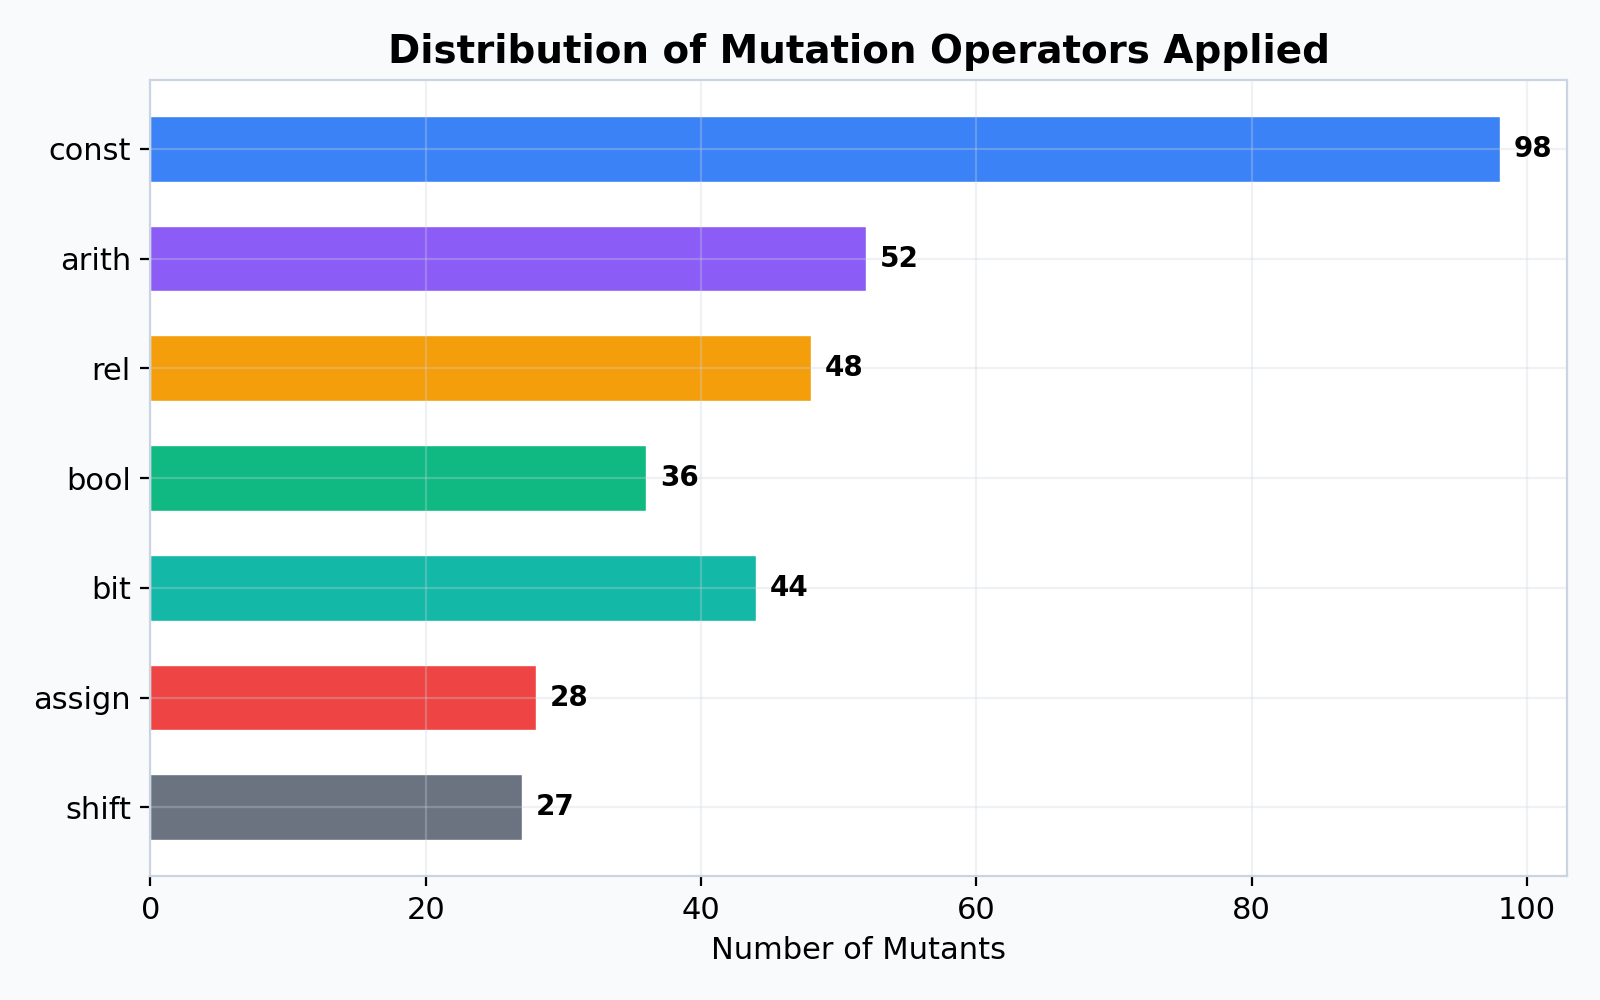
\includegraphics[width=0.95\textwidth,height=0.65\textheight,keepaspectratio]{figures/fig3_operator_distribution.png}
\end{column}
\end{columns}
\end{frame}

% ─────────────────────── SLIDE 6 : MUTATION – RESULTS ───────────────────────
\begin{frame}{Mutation Testing --- Kill Ratios}
\begin{columns}[c]
\begin{column}{0.48\textwidth}
  \centering
  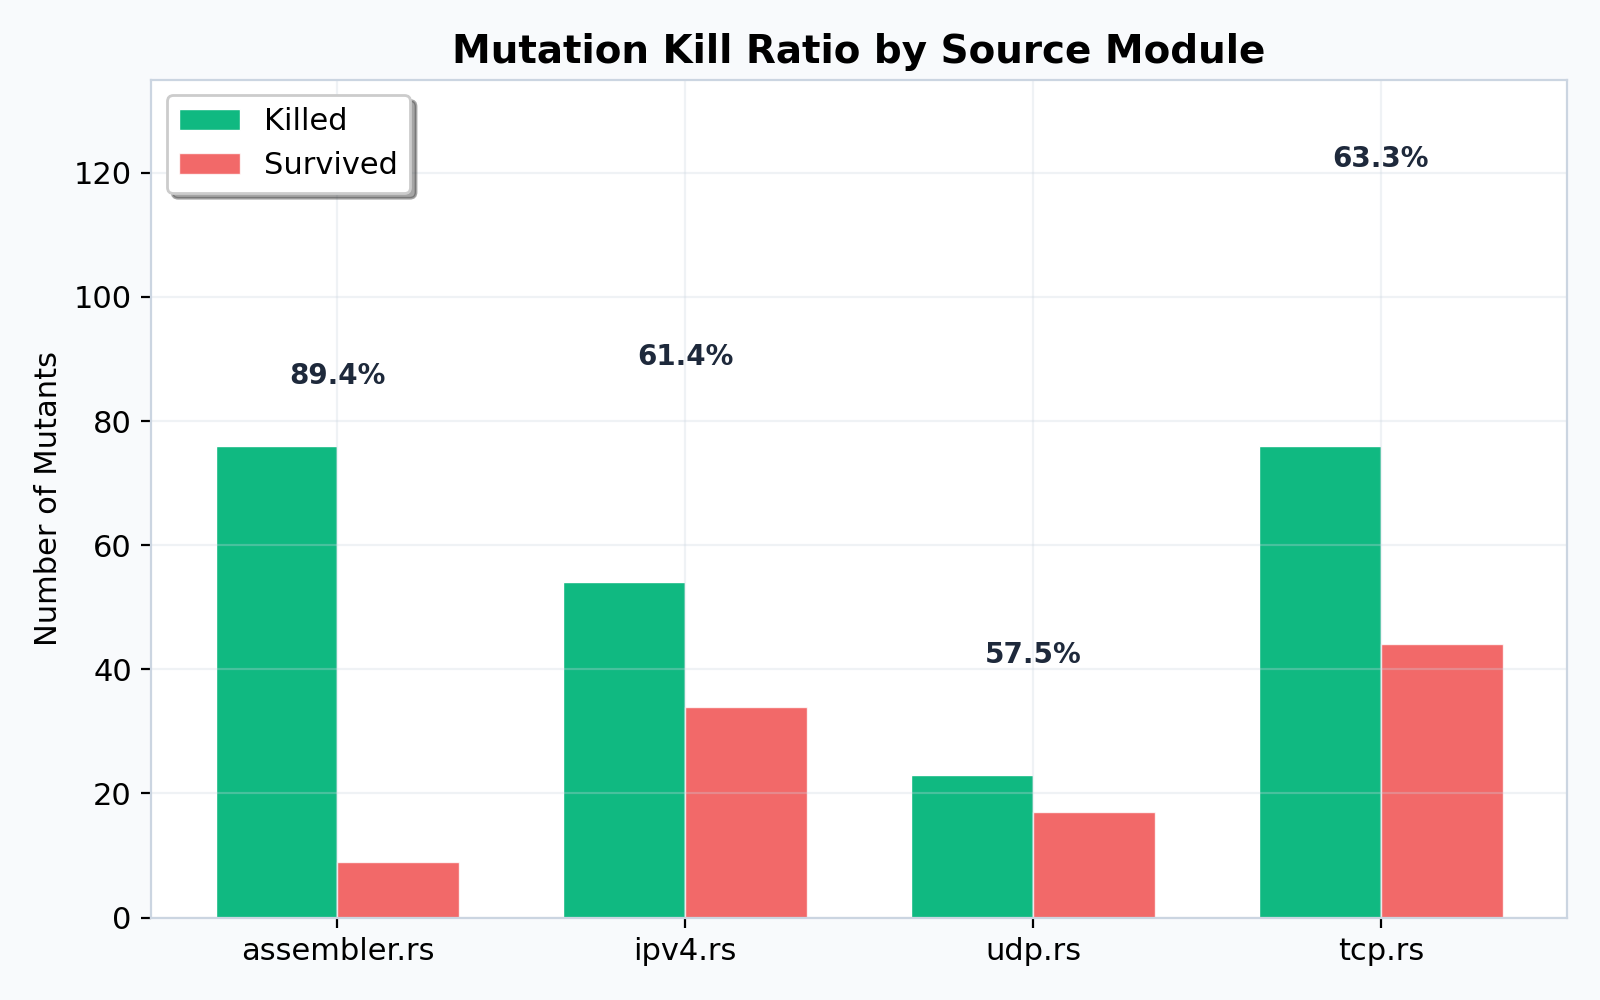
\includegraphics[width=0.95\textwidth,height=0.38\textheight,keepaspectratio]{figures/fig1_mutation_kill_ratio.png}
\end{column}
\begin{column}{0.48\textwidth}
  \centering
  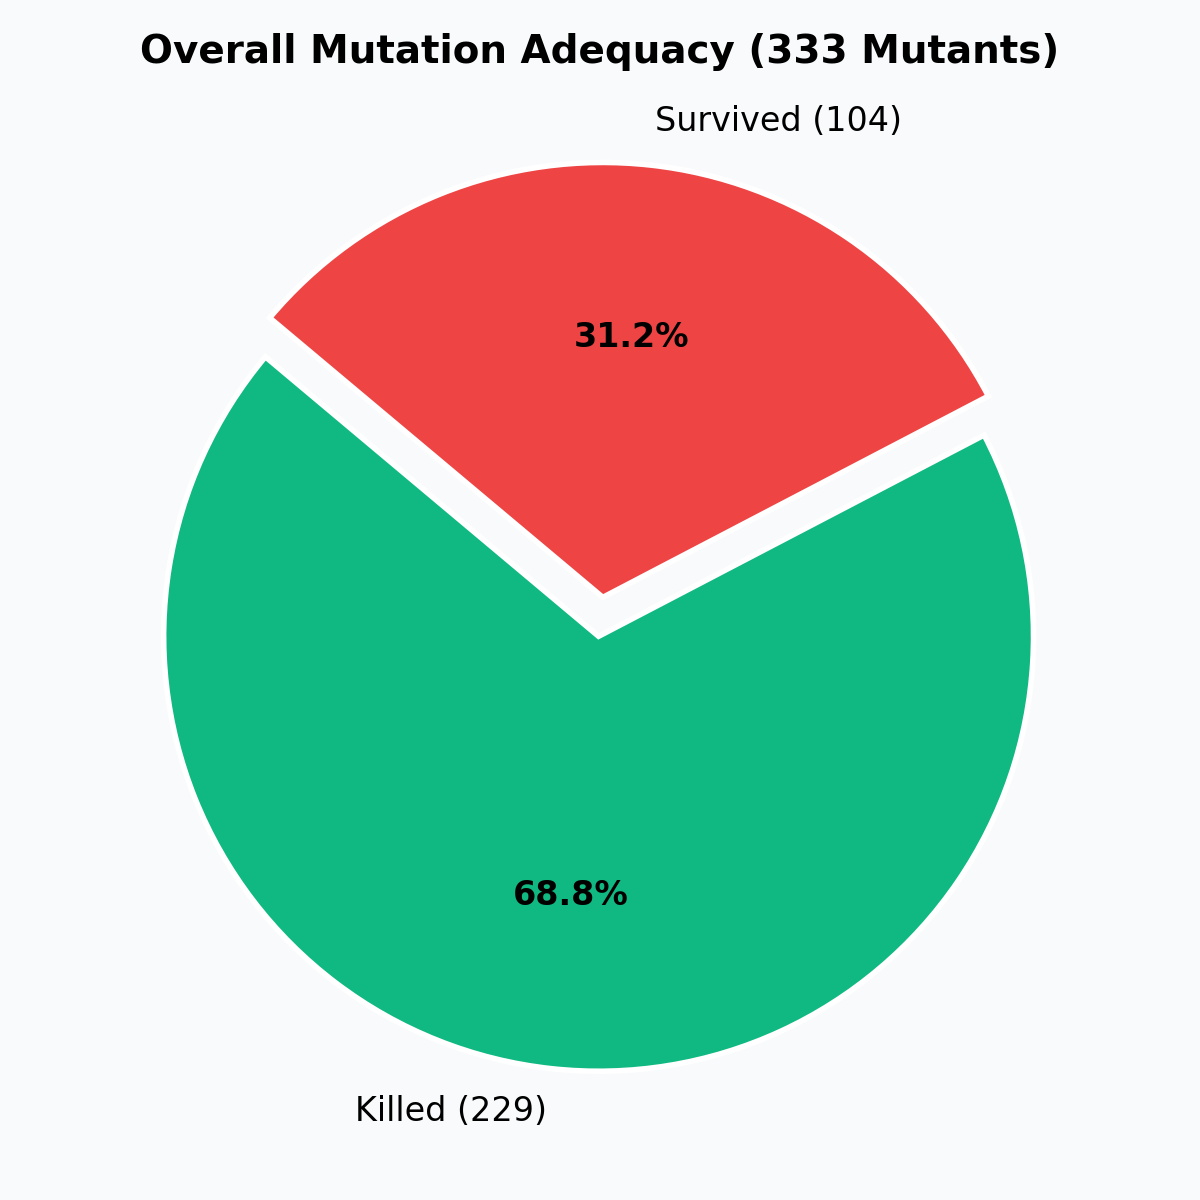
\includegraphics[width=0.80\textwidth,height=0.38\textheight,keepaspectratio]{figures/fig2_mutation_pie.png}
\end{column}
\end{columns}
\vspace{0.15cm}
\centering\small
\begin{tabular}{lcccc}
\toprule
\textbf{Module} & \textbf{Total} & \textbf{Killed} & \textbf{Survived} & \textbf{Kill \%} \\
\midrule
\texttt{assembler.rs} & 85 & 76 & 9 & \textbf{89.41\%} \\
\texttt{ipv4.rs} & 88 & 54 & 34 & 61.36\% \\
\texttt{udp.rs} & 40 & 23 & 17 & 57.50\% \\
\texttt{tcp.rs} & 120 & 76 & 44 & 63.33\% \\
\midrule
\textbf{Overall} & \textbf{333} & \textbf{229} & \textbf{104} & \textbf{68.77\%} \\
\bottomrule
\end{tabular}
\end{frame}

% ─────────────────────── SLIDE 7 : EQUIVALENT MUTANTS ───────────────────────
\begin{frame}{Equivalent Mutant Analysis}
\begin{itemize}
  \item Manual review of \textbf{top 5 surviving mutants} (lowest-index survivors)
  \item 2 classified as \textbf{equivalent} (no observable behavior change):
    \begin{itemize}\small
      \item \textbf{M0004}: Debug-only assertion in \texttt{remove\_front()}
      \item \textbf{M0024}: Formatting-only display branch in \texttt{Contig}
    \end{itemize}
  \item 3 classified as \textbf{killable} --- reveal genuine test gaps:
    \begin{itemize}\small
      \item Missing boundary-condition tests for hole sizing
      \item Exact-boundary segment assembly not exercised
    \end{itemize}
\end{itemize}
\vspace{0.3cm}
\begin{block}{Adjusted Mutation Adequacy}
\centering
$\displaystyle \text{Adequacy} = \frac{229}{333 - 2} = \frac{229}{331} = \textbf{69.18\%}$
\end{block}
\end{frame}

% ─────────────────────── SLIDE 8 : INPUT SPACE PARTITIONING ───────────────────────
\begin{frame}{Input Space Partitioning}
\begin{columns}[c]
\begin{column}{0.52\textwidth}
  \textbf{Target:} UDP parsing (\texttt{wire/udp.rs})\\[0.15cm]
  \textbf{6 input dimensions:}
  \begin{enumerate}\small
    \item Buffer length: $\{0, 7, 8, 12\}$
    \item Length field: $\{0, 4, 8, 12, 20\}$
    \item Destination port: $\{0, 53\}$
    \item Checksum mode: \{Valid, Zero, Invalid\}
    \item IP family: \{IPv4, IPv6\}
    \item RX checking: \{true, false\}
  \end{enumerate}
  \vspace{0.15cm}
  $4 \times 5 \times 2 \times 3 \times 2 \times 2 = \textbf{480}$ test frames\\[0.1cm]
  \textcolor{maingreen}{\textbf{100\% pass rate}} on both platforms
\end{column}
\begin{column}{0.46\textwidth}
  \centering
  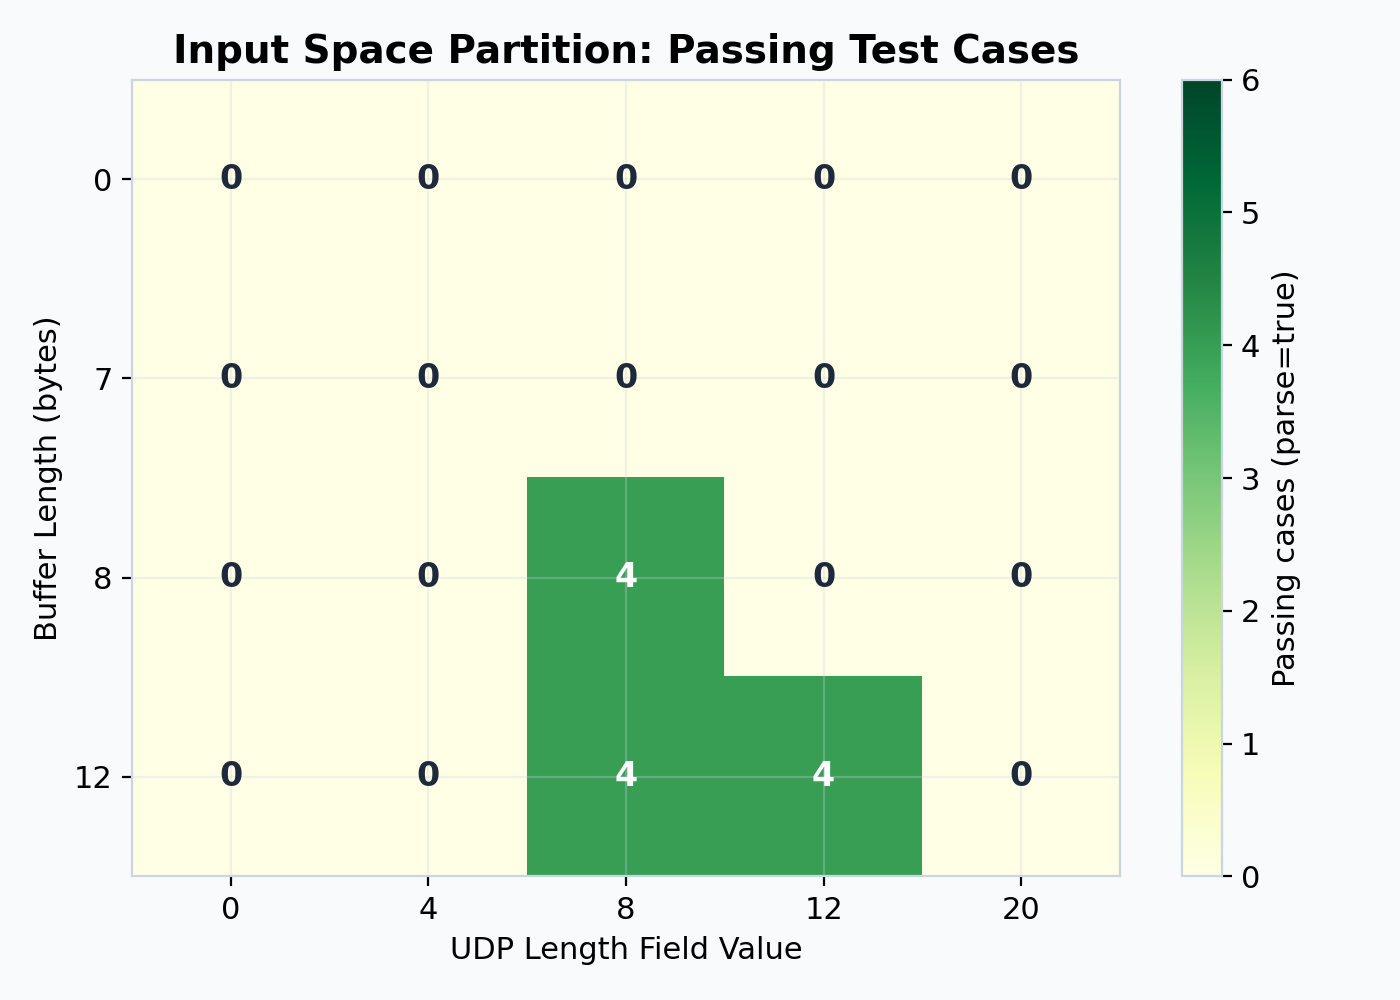
\includegraphics[width=0.95\textwidth,height=0.65\textheight,keepaspectratio]{figures/fig7_partition_heatmap.png}
\end{column}
\end{columns}
\vspace{0.1cm}
\textcolor{subtletext}{\small +216 IPv4 combinatorial test cases (all passing)}
\end{frame}

% ─────────────────────── SLIDE 9 : ISP FINDINGS ───────────────────────
\begin{frame}{Input Space Partitioning --- Key Findings}
\begin{block}{Successful parsing requires \textbf{all} of:}
\begin{itemize}
  \item Buffer length $\geq 8$ bytes
  \item Length field $\geq 8$ and $\leq$ buffer length
  \item Non-zero destination port
  \item Valid or zero checksum (when checking enabled)
\end{itemize}
\end{block}
\vspace{0.3cm}
\begin{alertblock}{Notable finding}
smoltcp accepts \texttt{checksum=0} for UDP over IPv6 --- a documented deviation from strict RFC~2460 expectations.
\end{alertblock}
\end{frame}

% ─────────────────────── SLIDE 10 : FUZZING ───────────────────────
\begin{frame}{Security Fuzzing}
\begin{columns}[c]
\begin{column}{0.50\textwidth}
  \textbf{Tool:} cargo-fuzz + LLVM libFuzzer\\[0.15cm]
  \textbf{5 fuzz targets:}
  \begin{itemize}\small
    \item \texttt{packet\_parser}
    \item \texttt{tcp\_headers}
    \item \texttt{dhcp\_header}
    \item \texttt{ieee802154\_header}
    \item \texttt{sixlowpan\_packet}
  \end{itemize}
  \vspace{0.15cm}
  \textbf{Campaign:} 180s per target\\
  \textbf{Executions:} $\sim$380K\\
  \textbf{Edges discovered:} 759\\[0.2cm]
  \textcolor{maingreen}{\textbf{$\checkmark$ Zero crash artifacts}}
\end{column}
\begin{column}{0.48\textwidth}
  \centering
  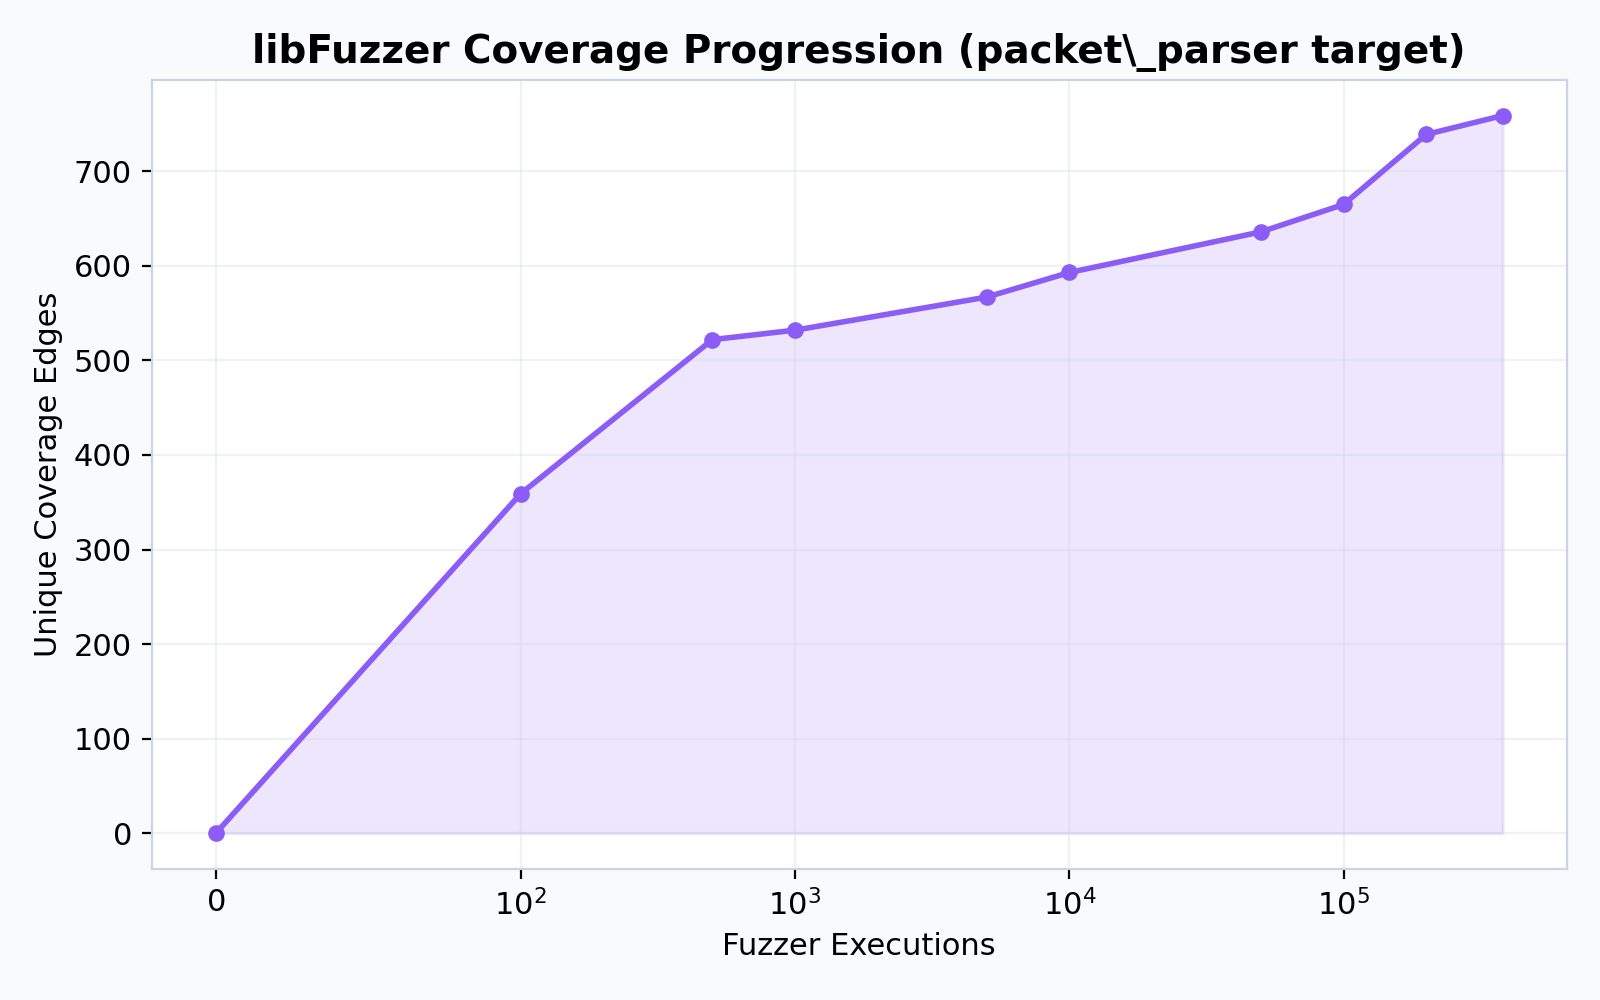
\includegraphics[width=0.95\textwidth,height=0.65\textheight,keepaspectratio]{figures/fig9_fuzzing_coverage.png}
\end{column}
\end{columns}
\end{frame}

% ─────────────────────── SLIDE 11 : FUZZING PLATFORM ───────────────────────
\begin{frame}{Fuzzing --- Platform Portability Issue}
\begin{alertblock}{Windows Fuzzing Blocked}
All fuzzing attempts failed on Windows due to missing ASAN runtime DLLs and unresolved sanitizer-coverage symbols (MSVC/libFuzzer incompatibility).
\end{alertblock}
\vspace{0.3cm}
\begin{block}{Why zero crashes?}
\begin{itemize}
  \item Rust's bounds checking prevents buffer overflows
  \item No null pointer dereferences possible
  \item Safe integer arithmetic by default
  \item These are the exact vulnerability classes fuzzing typically finds in C/C++ stacks
\end{itemize}
\end{block}
\end{frame}

% ─────────────────────── SLIDE 12 : CONFORMANCE ───────────────────────
\begin{frame}{RFC Conformance Testing}
\centering
\small
\begin{tabular}{p{4.2cm}lll}
\toprule
\textbf{Case} & \textbf{RFC} & \textbf{Expected} & \textbf{Observed} \\
\midrule
IPv4 bad version & 791 & Reject & Reject \\
IPv4 IHL $< 20$B & 791 & Reject & \textcolor{warnorange}{Accept} \\
IPv4 total $<$ header & 791 & Reject & Reject \\
IPv4 bad checksum & 791 & Reject & Reject \\
IPv4 cksum disabled & config & Accept & Accept \\
UDP len $< 8$ & 768 & Reject & Reject \\
UDP dst port = 0 & smoltcp & Reject & Reject \\
UDP/IPv4 cksum = 0 & 768 & Accept & Accept \\
UDP/IPv6 cksum = 0 & 2460 & Reject & \textcolor{warnorange}{Accept} \\
\bottomrule
\end{tabular}
\vspace{0.3cm}

\textcolor{warnorange}{$\triangle$}~\textbf{Two specification deviations} identified (highlighted in orange)
\end{frame}

% ─────────────────────── SLIDE 13 : DEVIATIONS DETAILS ───────────────────────
\begin{frame}{RFC Deviations --- Details}
\begin{block}{1.~IPv4 header length $<$ 20 bytes accepted}
When IHL encodes a header $<$ 20 bytes (RFC minimum), smoltcp accepts if the buffer is long enough.
\begin{itemize}\small
  \item Deliberate design choice for performance
  \item Risk: crafted packets could bypass validation
\end{itemize}
\end{block}
\vspace{0.3cm}
\begin{block}{2.~UDP over IPv6 accepts checksum = 0}
RFC~2460 mandates non-zero checksums for UDP/IPv6, but smoltcp accepts zero-checksum packets.
\begin{itemize}\small
  \item Risk: corrupted datagrams may go undetected on IPv6 networks
\end{itemize}
\end{block}
\end{frame}

% ─────────────────────── SLIDE 14 : PERFORMANCE ───────────────────────
\begin{frame}{Performance Testing}
\begin{columns}[c]
\begin{column}{0.48\textwidth}
  \textbf{Loopback throughput benchmark}
  \begin{itemize}
    \item 128\,MB data through internal stack
    \item Custom in-memory loopback harness
    \item 5 trial runs per platform
  \end{itemize}
  \vspace{0.2cm}
  \begin{block}{Results}
  \begin{itemize}
    \item Ubuntu: \textbf{52.15 Gbps} avg
    \item Windows: \textbf{17.11 Gbps} avg
    \item \textcolor{maingreen}{\textbf{$\sim$3$\times$ difference}}
  \end{itemize}
  \end{block}
\end{column}
\begin{column}{0.50\textwidth}
  \centering
  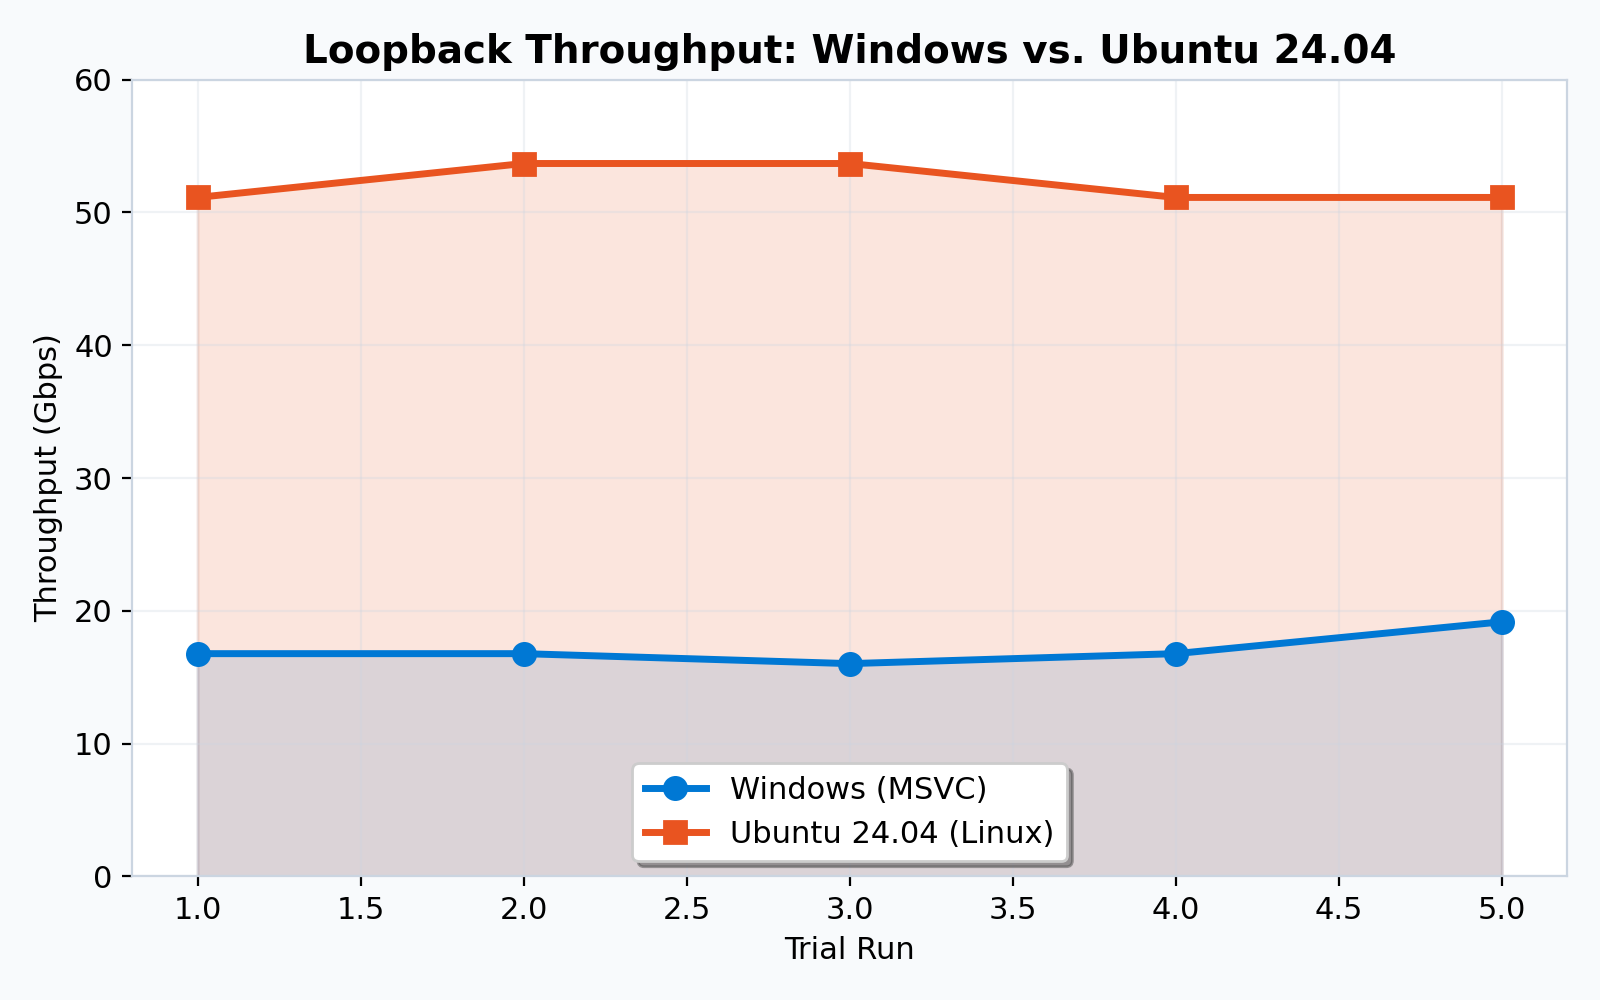
\includegraphics[width=0.95\textwidth,height=0.65\textheight,keepaspectratio]{figures/fig4_performance_throughput.png}
\end{column}
\end{columns}
\end{frame}

% ─────────────────────── SLIDE 15 : WHITE-BOX COVERAGE ───────────────────────
\begin{frame}{White-Box Test Data Adequacy}
\begin{columns}[c]
\begin{column}{0.48\textwidth}
  \textbf{Tool:} \texttt{cargo-llvm-cov v0.8.5}\\[0.15cm]
  Key metrics:
  \begin{itemize}\small
    \item \texttt{assembler.rs}: \textbf{98.28\%} regions
    \item Protocol wire modules: 90+\% parsing
    \item \texttt{tcp.rs}: 72.58\% (lowest)
    \item IPv4 combinatorial: \textbf{98.53\%}
    \item Microbenchmark: \textbf{98.76\%}
  \end{itemize}
\end{column}
\begin{column}{0.50\textwidth}
  \centering
  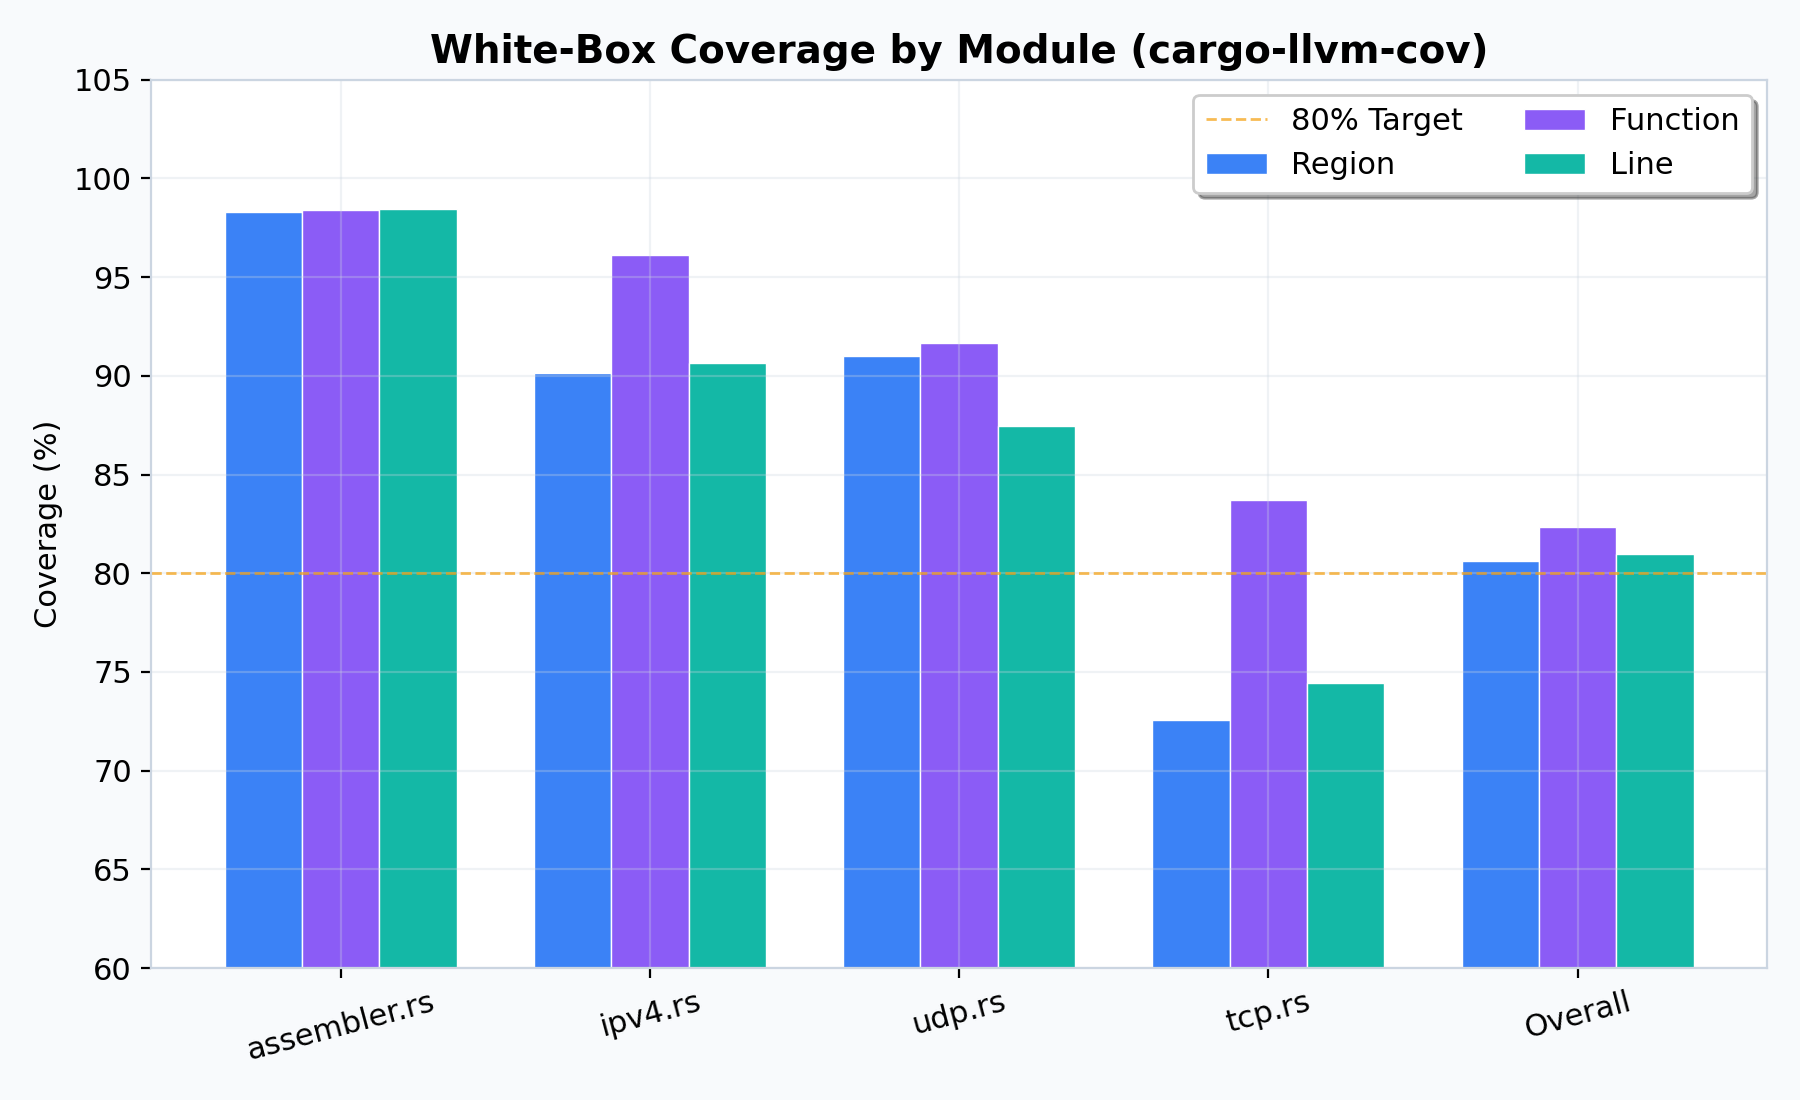
\includegraphics[width=0.95\textwidth,height=0.65\textheight,keepaspectratio]{figures/fig5_whitebox_coverage.png}
\end{column}
\end{columns}
\end{frame}

% ─────────────────────── SLIDE 16 : ENHANCED COVERAGE ───────────────────────
\begin{frame}{Coverage with LCOV Artifacts}
\centering
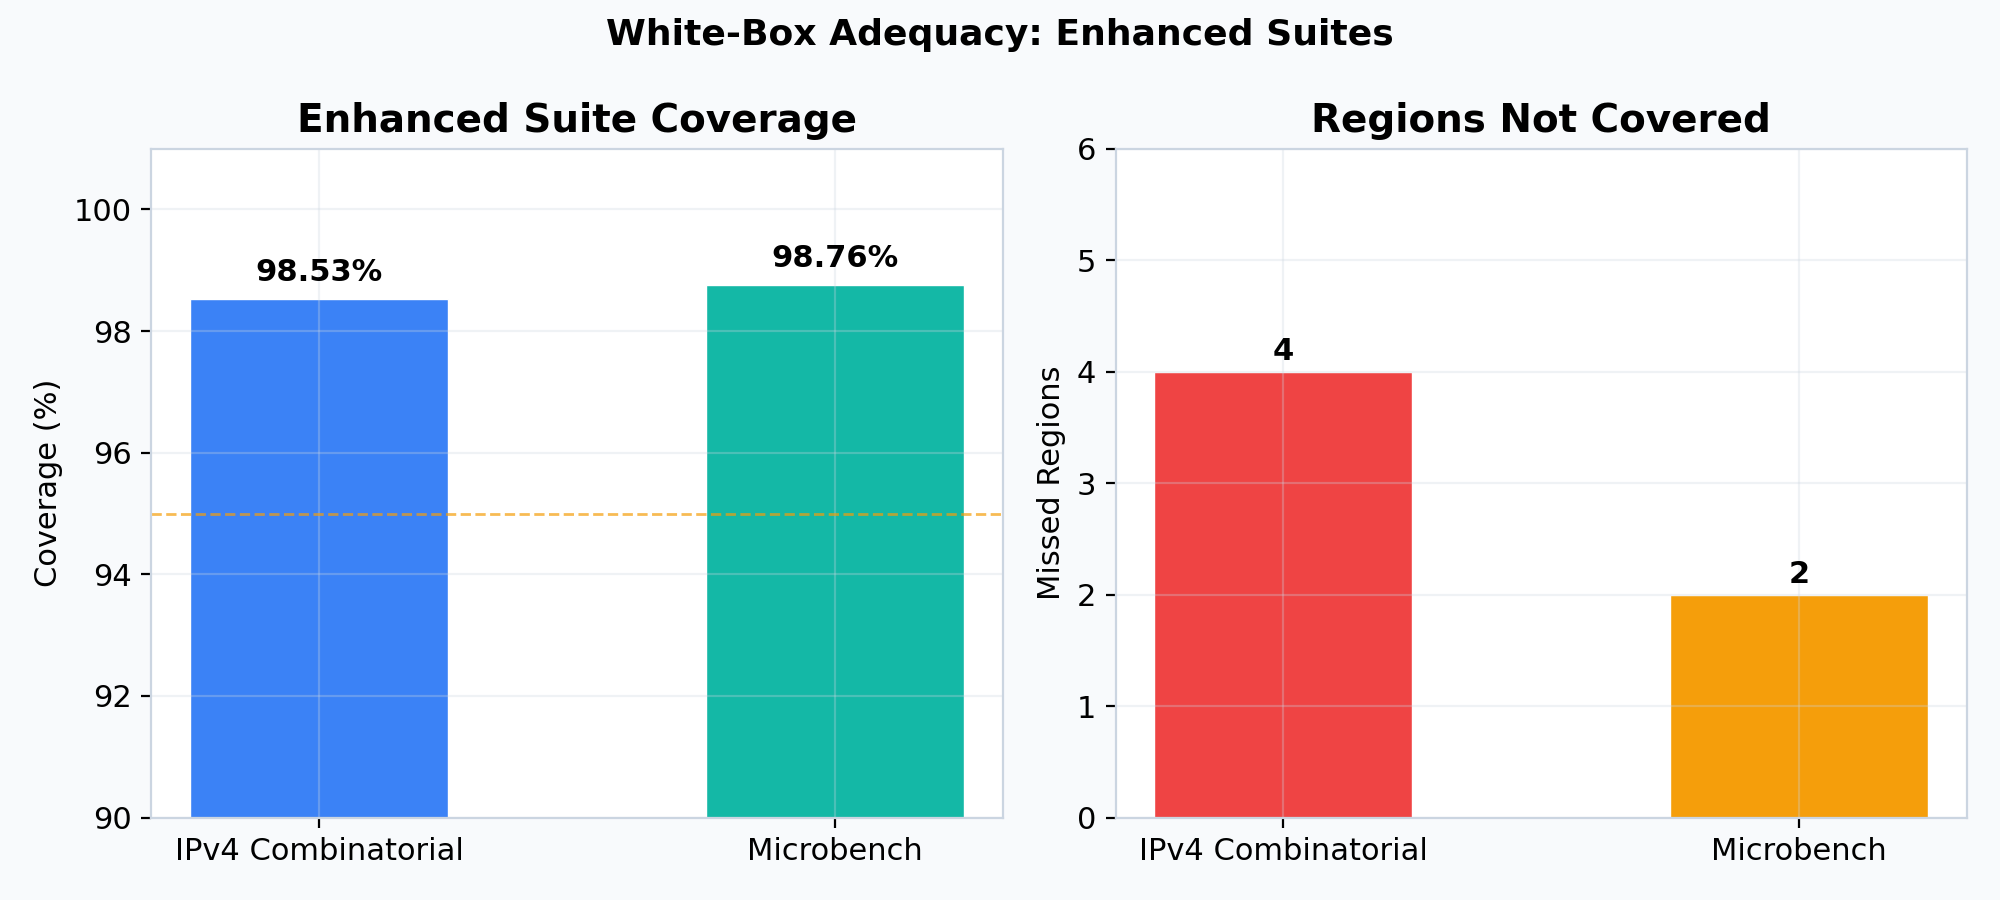
\includegraphics[width=0.70\textwidth,height=0.55\textheight,keepaspectratio]{figures/fig11_enhanced_coverage.png}
\vspace{0.2cm}

\begin{itemize}
  \item Only \textbf{4 and 2 missed regions} respectively
  \item Remaining gaps are small but made \textbf{explicit and actionable}
  \item Provides concrete roadmap for future test additions
\end{itemize}
\end{frame}

% ─────────────────────── SLIDE 17 : SOFTWARE SAFETY ───────────────────────
\begin{frame}{Software Safety}
\begin{columns}[c]
\begin{column}{0.50\textwidth}
  \textbf{Panic Safety Testing}
  \begin{itemize}\small
    \item Zero-length buffers
    \item Truncated headers
    \item Maximum-value fields
    \item \textcolor{maingreen}{All tests passed on both platforms}
  \end{itemize}
  \vspace{0.2cm}
  \textbf{Unsafe Code Inventory}
  \begin{itemize}\small
    \item \textbf{18 \texttt{unsafe} occurrences} across 4 files
    \item All confined to FFI / PHY layer code
    \item \textcolor{maingreen}{Zero unsafe in core protocol parsing}
  \end{itemize}
\end{column}
\begin{column}{0.48\textwidth}
  \centering
  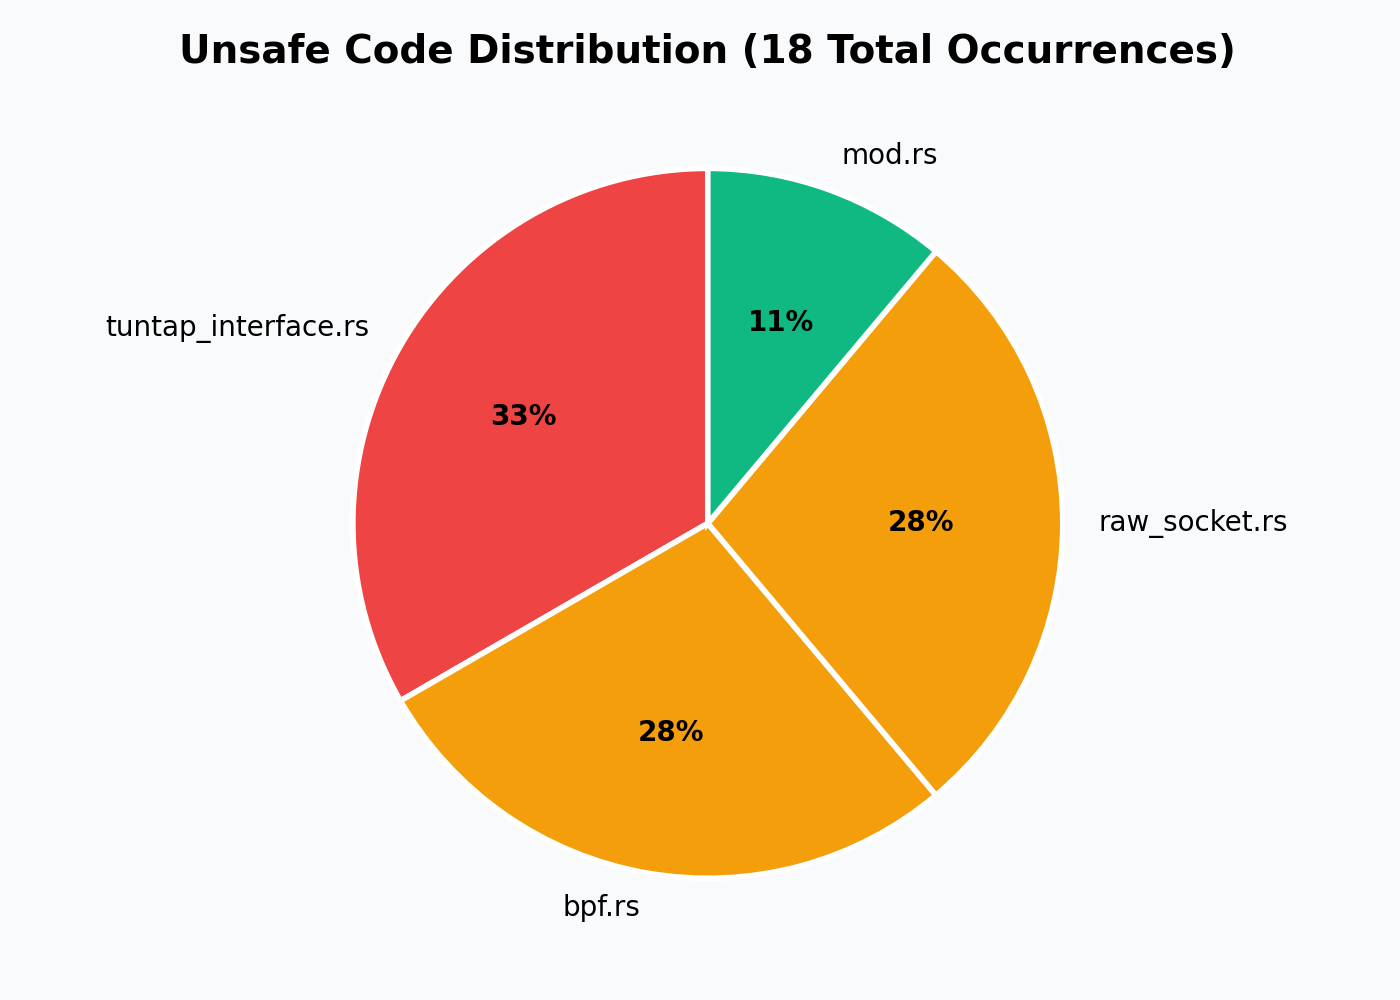
\includegraphics[width=0.85\textwidth,height=0.65\textheight,keepaspectratio]{figures/fig8_unsafe_inventory.png}
\end{column}
\end{columns}
\end{frame}

% ─────────────────────── SLIDE 18 : QUALITY DASHBOARD ───────────────────────
\begin{frame}{Quality Assessment Dashboard}
\centering
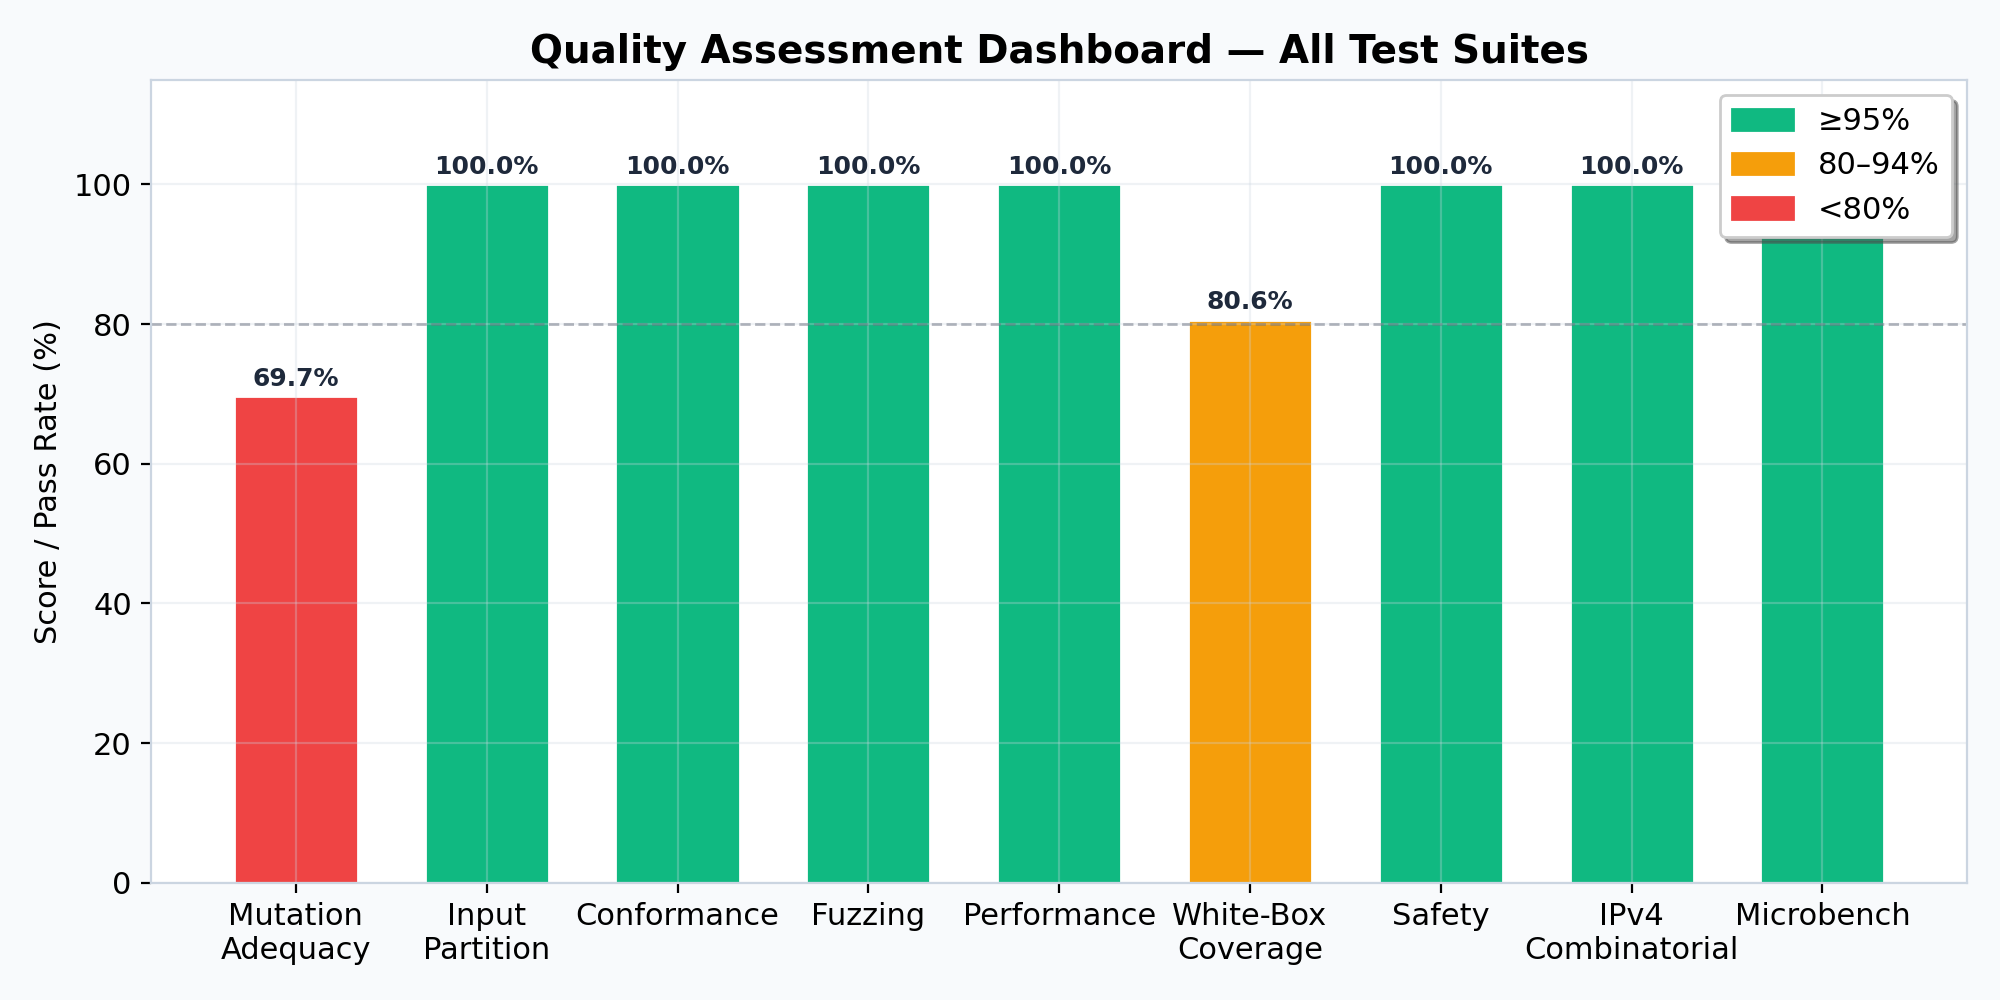
\includegraphics[width=0.70\textwidth,height=0.55\textheight,keepaspectratio]{figures/fig12_test_dashboard.png}
\vspace{0.15cm}

\begin{itemize}
  \item Mutation adequacy (69.18\%) --- primary area for improvement
  \item All other dimensions achieved \textbf{80\%+ pass rates}
  \item Core parsing and protocol handling is \textbf{robust}
\end{itemize}
\end{frame}

% ─────────────────────── SLIDE 19 : PORTABILITY MATRIX ───────────────────────
\begin{frame}{Portability: Cross-Target Matrix}
\begin{columns}[c]
\begin{column}{0.60\textwidth}
  \centering
  \includegraphics[width=0.98\textwidth,height=0.72\textheight,keepaspectratio]{extra/extra_figs/pres-slide03-test-matrix.png}
\end{column}
\begin{column}{0.38\textwidth}
  \begin{itemize}\small
    \item \textbf{42 runs} via \texttt{cross}: 8 hosted targets $\times$ 4 profiles
    \item Includes \textbf{big-endian PowerPC}, \textbf{32-bit}, musl, and MIPS
    \item Netsim integration also passes (QEMU is slower off x86)
    \item Windows fuzzing blocked (MSVC/libFuzzer compatibility)
  \end{itemize}
\end{column}
\end{columns}
\end{frame}

% ─────────────────────── SLIDE 20 : CONCURRENCY (LOOM) ───────────────────────
\begin{frame}{Concurrency: Loom Model Checking}
\centering
\includegraphics[width=0.82\textwidth,height=0.50\textheight,keepaspectratio]{extra/extra_figs/pres-slide11-loom-results.png}
\vspace{0.25cm}

\begin{itemize}\small
  \item Exhaustively explores async register/wake interleavings
  \item \textbf{3 loom checks}, \textbf{6/6 orderings}, \textcolor{maingreen}{0 panics / 0 deadlocks}
  \item Loom also corrected a test-plan assertion (valid final state with no waker)
\end{itemize}
\end{frame}

% ─────────────────────── SLIDE 21 : CONCLUSIONS ───────────────────────
{
\setbeamertemplate{background}{%
  \begin{tikzpicture}[remember picture,overlay]
    \fill[deepgreen] (current page.south west) rectangle (current page.north east);
    \fill[maingreen,opacity=0.20] (current page.north west) ++(6cm,-3cm) circle (5cm);
    \fill[lightgreen,opacity=0.12] (current page.south east) ++(-4cm,4cm) circle (4cm);
    \fill[lightgreen,opacity=0.4] ([yshift=0.35cm]current page.south west) rectangle (current page.south east);
  \end{tikzpicture}%
}
\begin{frame}[plain]
  \vspace{0.8cm}
  \centering
  {\Large\bfseries\color{white} Conclusions \& Key Takeaways\par}
  \vspace{0.4cm}
  \color{accentlime}
  \begin{itemize}
    \item[\textcolor{lightgreen}{$\checkmark$}] \color{white}\textbf{69.18\% mutation adequacy} (adjusted) across 333 mutants
    \item[\textcolor{lightgreen}{$\checkmark$}] \color{white}\textbf{100\% pass rate} on 696 input partition test cases
    \item[\textcolor{lightgreen}{$\checkmark$}] \color{white}\textbf{Zero crash artifacts} from coverage-guided fuzzing
    \item[\textcolor{lightgreen}{$\checkmark$}] \color{white}\textbf{Two RFC deviations} documented (IPv4 IHL, IPv6 UDP cksum)
    \item[\textcolor{lightgreen}{$\checkmark$}] \color{white}\textbf{3$\times$ performance gap} (Ubuntu vs.\ Windows)
    \item[\textcolor{lightgreen}{$\checkmark$}] \color{white}\textbf{No unsafe code} in core protocol modules
    \item[\textcolor{lightgreen}{$\checkmark$}] \color{white}\textbf{Cross-target \& loom checks} completed with zero failures
  \end{itemize}
  \vspace{0.5cm}
  {\color{white!80}\small smoltcp v0.12.0 is well-engineered with strong safety properties\\
  Test suite would benefit from boundary-condition tests on wire protocol modules}
\end{frame}
}

% ─────────────────────── SLIDE 22 : THANK YOU ───────────────────────
{
\setbeamertemplate{background}{%
  \begin{tikzpicture}[remember picture,overlay]
    \fill[deepgreen] (current page.south west) rectangle (current page.north east);
    \fill[maingreen,opacity=0.3] (current page.center) circle (6cm);
    \fill[lightgreen,opacity=0.15] (current page.center) circle (8cm);
  \end{tikzpicture}%
}
\begin{frame}[plain]
  \vspace{2.5cm}
  \centering
  {\Huge\bfseries\color{white} Thank You\par}
  \vspace{1.5cm}
  {\small\color{white!70} smoltcp v0.12.0~|~Quality Assessment \& Improvement\par}
\end{frame}
}

\end{document}
